%\usepackage{nicematrix}






% \section{Introduction}

In this chapter we summarize the available geological, mechanical, and hydraulic data for \URFBII that will be used in the inversion of the pore-pressure experiment (Chapters \ref{ch:model_comparison}--\ref{ch:inversion}) and in the transport model for the \Gls{EDZ} (Chapter \ref{ch:transport}).
The primary sources are S\'URAO technical reports, mainly those produced within the projects \textquote{Geological and geotechnical characterisation of the rock environment -- \URFBII} (hereafter referred to as the \textquote{Characterization project}), \textquote{Stanovení in-situ napjatosti v PVP Bukov II} (Stress Assessment), and \textquote{Data Acquisition from the Deep Horizons of the Rožná Mine} (Deep Horizons).

% Charakterizace Bukova II - označení chodeb, rozrážek a vrtů
% \URFBII is located on level 12 of the \Rozna in the Czech Republic, approximately at sea level, that is 500--600 meters below Earth's surface.

% For hydrological, mechanical, and coupled models of this zone, physical parameters need to be set according to available measurements and experimental analyses.


%%% preneseno z uvodu kap. od Felipeho

\section{Geological context}
\label{sec_geology}

% \sts{[S: Doporucil bych celou sekci \ref{sec_geology} presunout nekam do treti kapitoly.]}

\par The geological context of the \URFBII is rooted in the complex geomechanics of the 12\textsuperscript{th} level of the 
% \href{https://www.google.com/url?sa=t&rct=j&q=&esrc=s&source=web&cd=&ved=2ahUKEwj_x4Xo1OaOAxWpQ_EDHYluA8IQFnoECB4QAQ&url=https%3A%2F%2Fmineralexpert.org%2Farticle%2Frozna-uranium-mine&usg=AOvVaw0CJNZxChFCpxJT_Fe9Y5V7&opi=89978449}{Rožná} 
\Rozna mine in the Czech Republic, situated approximately 500--600 meters below the earth's surface.
The research facility consists of several galleries, each approximately 70--90 m long, accessed from the main transport gallery P\v S1-123, see Fig. \ref{fig:mapa}.
\begin{figure}
    \centering
    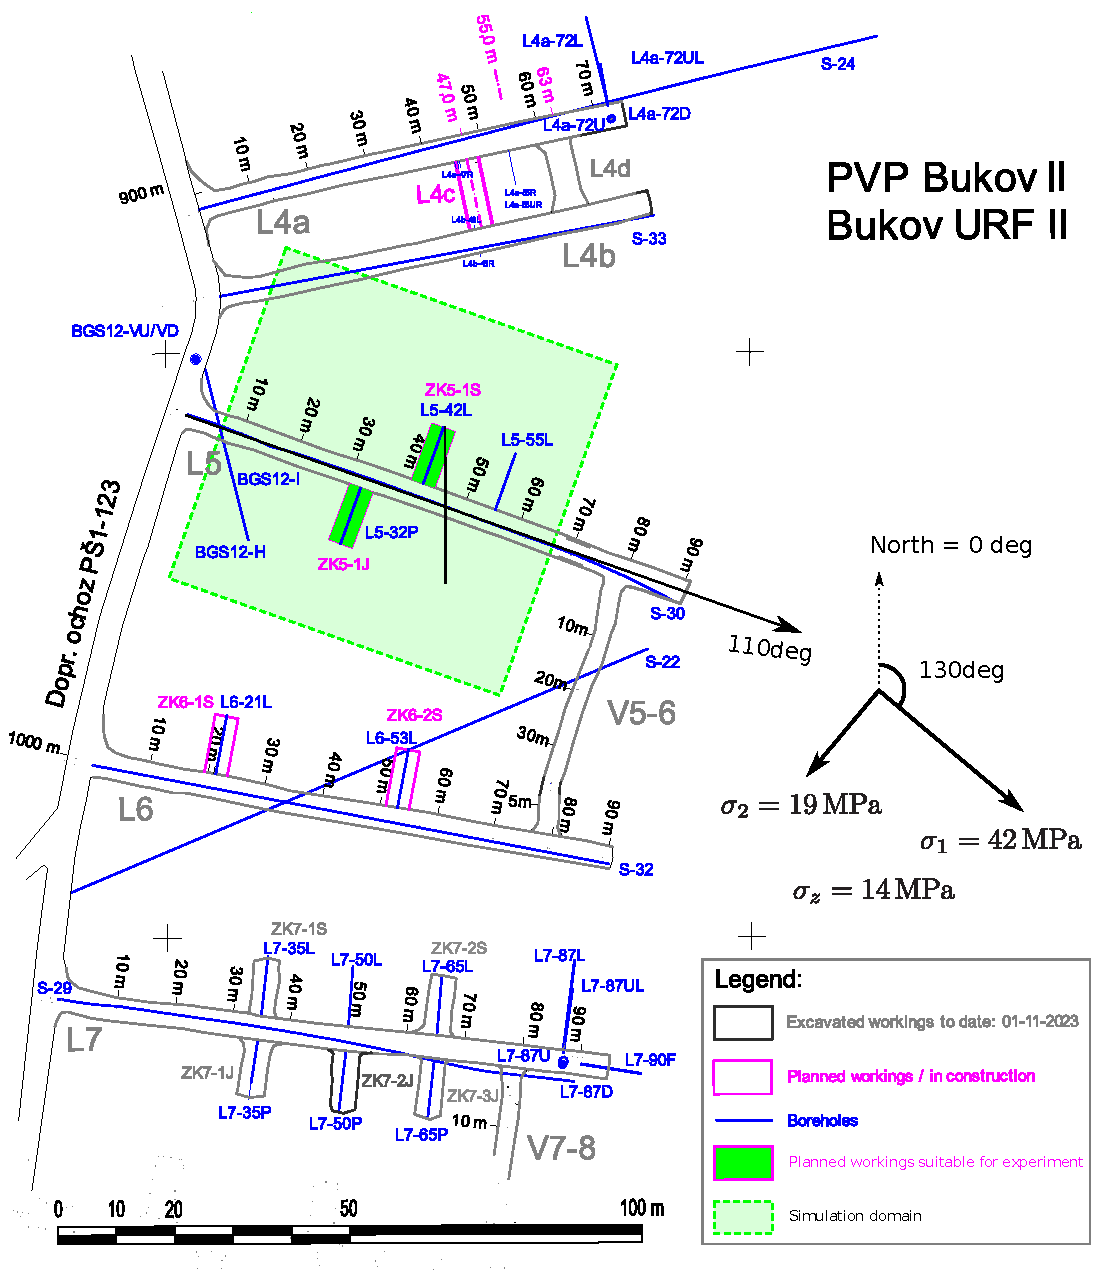
\includegraphics[width=\textwidth]{graphics/mapa_en.pdf}
    \caption{Situation plan of \URFBII.}
    \label{fig:mapa}
\end{figure}
The zone of interest is around the L5 laboratory gallery and the adjacent 10 m long ZK5-1J and ZK5-1S test chambers.


\par The geology here is heavily influenced by metamorphic processes, with structural foliation affecting mechanical and hydraulic properties.

\par Mechanically, the rock mass exhibits properties influenced by its foliation, as evidenced by uniaxial, cyclic loading, and triaxial tests performed on core samples. The elastic modulus varies considerably based on orientation relative to foliation (orthogonal, parallel, or skewed). Measurements include deformation modulus values up to 71.9 GPa and uniaxial compressive strengths reaching 231 MPa (\cite{Bukovska2025}). 
\par Cyclic and triaxial tests revealed complex stress-strain behavior, with the Hoek-Brown criterion providing a framework for strength characterization.


\paragraph{Geological materials.}
% \subsection{Geological Model and Lithologies}
% The numerical model incorporates a new mesh derived from a highly detailed 

According to a detailed geological model created by the Czech Geological Survey (\cite{Bukovska2025final}), the lithologies present at the site primarily include:
\begin{itemize}%[noitemsep]
    \item Migmatitized amphibolite,
    \item Migmatite,
    \item Biotite-Amphibole paragneiss migmatitized.
\end{itemize}
An illustration of the material layout in the surrounding of the \gls{L5} is depicted in Fig. \ref{fig:geological_mesh}.

\begin{figure}%[H]
    \centering
    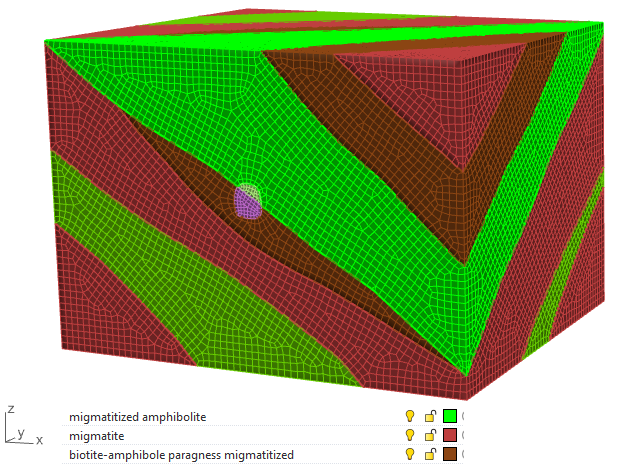
\includegraphics[width=0.5\textwidth]{graphics/plasticity/geological_mesh.png} % Example image path
    % \caption{Mesh used in this study compromising the detailed geological setting.}
    \caption{Structure of geological materials in the zone of interest.}
    \label{fig:geological_mesh}
\end{figure}


%%% po sem preneseno z kap. od Felipeho


\section{Mechanical parameters}\label{sec:review_mech}

% \sts{[S: Asi by bylo vhodne take zohlednit materialovou heterogenitu zminenou vyse, viz sekce 3.1.2.]}

Within the Characterization project (see \cite{tz_char_1,tz_char_2,tz_char_3}), mechanical properties were investigated on samples from the L6, L7 and partially L5 and L8 galleries, using uniaxial compression, Brazilian test, cyclic loading, and triaxial tests.
In the Deep Horizons project (see \cite{tz_hh}), similar tests were done on samples from the 12\textsuperscript{th}--24\textsuperscript{th} level; moreover, in situ measurements of elastic moduli by the Goodman-Jack method were performed in boreholes at the mentioned levels.

We collected data from the following measurements:
\begin{itemize}
    \item Uniaxial compression tests and Brazilian tests on core samples from the L5--L8 galleries, as well as from a large-volume sample and boreholes located near \URFBII. The results include uniaxial compressive strength $\sigma_{pd}$, deformation modulus for $20-40~\%$ of maximal load $E_{20~\%-40~\%}$, Poisson's number $\mu$ and transversal tensile strength $\sigma_{ptp}$. See Tab. \ref{tab:mech_uniax} for the data and source citations.

    \item Cyclic loading tests on core samples from the L6--L7 galleries, as well as from a large-volume sample and boreholes located near \URFBII. The results include uniaxial compressive strength ($\sigma_{pd}$), deformation modulus in the first and second cycle, respectively ($E_{1def}$, $E_{2def}$), and elastic modulus in the first and second cycle, respectively ($E_{1el}$, $E_{2el}$). See Tab. \ref{tab:mech_cyclic} for the data and source citations.

    \item Triaxial tests on core samples from the L6--L7 galleries, as well as from a large-volume sample and boreholes located near \URFBII. The results include several lateral/axial stress measurements. See Tab. \ref{tab:mech_triax} for the data and source citations.

    \item In situ tests using the Goodman-Jack method on boreholes in \URFBII. The results include deformation moduli $E_{calc}$ as well as corrected values obtained from nomogram (ASTM 2016). See Tab. \ref{tab:goodman-jack}. According to Tab. 152 in \cite{tz_hh}, the average elastic modulus for the 12\textsuperscript{th} level is $18.3$ \unit\GPa.

    \item Some measurements were distinguished by the orientation relative to foliation (orthogonal (K), parallel (P) and skew (S)).
\end{itemize}


\paragraph{Rock mass moduli for the zone of interest.}
Besides the above data, the rock mass properties have been determined for the geologic materials that are present in the vicinity of the L5 gallery.

The rock mass modulus ($E_{rm}$) is obtained from the intact modulus $E_i$ and the rock mass quality parameters, i.e. the Geological Strength Index ($GSI$) and the disturbance factor ($D$), see (\cite{hoek2019hoek}), using the following formula:
$$
E_{rm} = E_i \left[ 0.02 + \frac{1 - \frac{D}{2}}{1 + \exp \left( \frac{60 + 15D - GSI}{11} \right)} \right]
$$
For this locality, a value of $GSI = 88$ and $D=0$ has been considered, according to the lowest GSI value mapped in the study site.
The rock mass moduli for the particular geological materials are summarized in \hyperref[tab:hoek_brown_summary_improved]{Table~\ref{tab:hoek_brown_summary_improved}}.


\paragraph{Hoek-Brown strength envelope parameters.}
The Hoek-Brown criterion is an empirical nonlinear failure criterion for isotropic rock masses, which incorporates the Geological Strength Index ($GSI$) and the disturbance factor ($D$) (see \cite{hoek2019hoek}).

The generalized Hoek-Brown failure criterion is given by:
\begin{equation}\label{eq:hoek-brown}
\sigma_1 = \sigma_3 + \sigma_{ci} \left( m_b \frac{\sigma_3}{\sigma_{ci}} + s \right)^a
\end{equation}
where:
\begin{itemize}%[noitemsep]
    \item $\sigma_1$ is the major principal stress,
    \item $\sigma_3$ is the minor principal stress,
    \item $\sigma_{ci}$ is the uniaxial compressive strength (UCS) of the intact rock,
    \item $m_b$, $s$, and $a$ are rock mass parameters.
\end{itemize}

These rock mass parameters are calculated from the intact rock properties ($m_i$, $\sigma_{ci}$) and the rock mass quality ($GSI$, $D$) by using the following equations:
$$
m_b = m_i \exp \left( \frac{GSI - 100}{28 - 14D} \right)
$$
$$
s = \exp \left( \frac{GSI - 100}{9 - 3D} \right)
$$
$$
a = \frac{1}{2} + \frac{1}{6} \left[ \exp \left( \frac{-GSI}{15} \right) - \exp \left( \frac{-20}{3} \right) \right]
$$
Considering the value of $GSI = 88$ and $D=0$, the above formulas give $s = 0.263597$ and $a = 0.50026$ for all lithologies.

The intact rock parameters, $\sigma_{ci}$ and $m_i$, have been determined within the Deep Horizons project from the laboratory measurements using the program RocData.
The corresponding parameters are given in Tab. \ref{tab:mech_stab}. 
% However, these data summarized from \cite{tz_hh} are incomplete because the Hoek-Brown model requires more than two parameters (see \cite{hoek2019hoek,hoek2002hoek}).
% In addition, these data were determined purely on basis of laboratory experiments and 
However, their modifications are necessary for in situ numerical simulations. The modifications can be done by empirical formulas introduced e.g. in \cite{hoek2019hoek,hoek2002hoek}). They were used in \cite{gong2021modelling} within numerical modelling in locality of the \Rozna.

Next, to obtain intact rock parameters appropriate for the considered locality, a fitting procedure was performed using triaxial data from migmatitized amphibolite and migmatite.

\par The fitting of the rock mass parameters was performed using a custom script developed in Python 3.12. The script applies a robust least-squares optimization to calibrate the Hoek-Brown failure criterion for intact rock, using laboratory triaxial test data.

The core of the methodology is the \verb|scipy.optimize.curve_fit| function, which performs a non-linear least squares fit. This process systematically minimizes the sum of the squared residuals, which represents the cumulative vertical distance between each data point and the fitted curve. The resulting parameters correspond to the mathematically optimal solution that produces the best possible fit to the provided data.

By focusing on minimizing the residuals, the procedure directly calibrates the fundamental Hoek-Brown parameters, Unconfined Compressive Strength ($\sigma_{ci}$) and the material constant ($m_i$), ensuring a scientifically defensible and quantitative representation of the rock's strength behavior.

There was no data for the  domain 'biotite-amphibole paragneiss migmatitized' and therefore, it has been assumed to have the same properties as of migmatitized amphibolite.

\begin{figure}%[H]
    \centering
    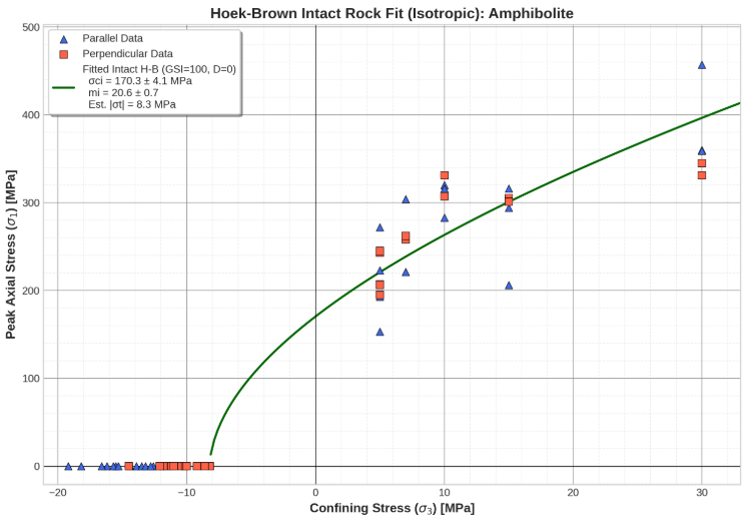
\includegraphics[width=0.9\textwidth]{graphics/plasticity/amphibolite_fit.png} % Example image path
    \caption{Hoek-Brown intact rock fit for amphibolite.}
    \label{fig:amphibolite_fit}
\end{figure}

\begin{figure}%[H]
    \centering
    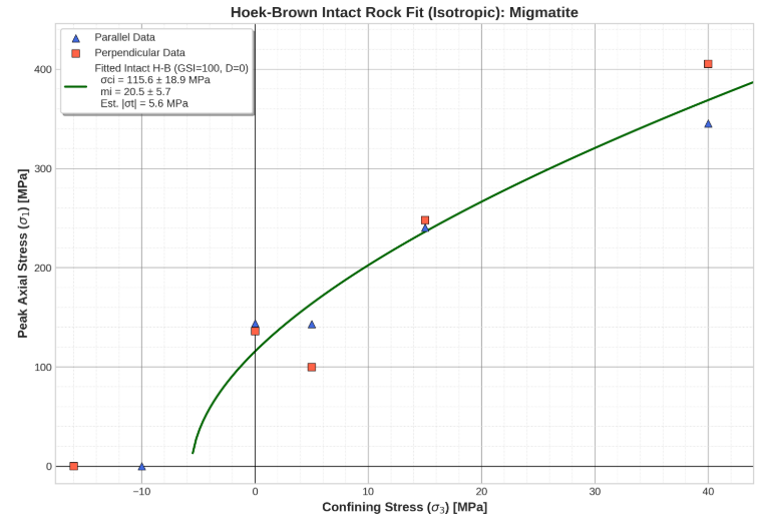
\includegraphics[width=0.9\textwidth]{graphics/plasticity/migmatite_fit.png} % Example image path
    \caption{Hoek-Brown intact rock fit for migmatite.}
    \label{fig:migmatite_fit}
\end{figure}

The results of the fit are summarized in \hyperref[tab:hoek_brown_summary_improved]{Table~\ref{tab:hoek_brown_summary_improved}}.




% \js{NOTE: 
% The Hoek-Brown plasticity model requires more than only two parameters (see \cite{hoek2019hoek,hoek2002hoek}). Some reference data can be found in the paper \cite{gong2021modelling} provided by S. Sysala. 
% Colleagues from IGN are welcome to update the review accordingly.}


\begin{table}[!htp]\centering
\caption{Mechanical parameters: Uniaxial tests.}\label{tab:mech_uniax}
\scriptsize
\begin{tabular}{@{}lccSSSSr@{}}\toprule
Location & Borehole &Orientation &$\sigma_{Pd}$ &{$E_{20-40~\%}$} &$\mu$ &$\sigma_{Ptp}$ &Data source \\%\cmidrule{1-8}
& /sample & &\unit\MPa &\unit\GPa &{--} &\unit\MPa & \\\midrule

\multirow{2}{*}{L7} &\multirow{2}{*}{16962} &K &231 &59.2 &0.19 &9 &\multirow{2}{*}{\cite{tz_char_1}, Tab. 16 $ $} \\
& &P &224 &71.9 &0.2 &14 & \\\midrule

\multirow{2}{*}{L8} &75328 &K &165.3 &62 &0.25 &16 &\multirow{2}{*}{\cite{tz_char_1}, Tab. 19 $ $} \\
&75329 &P &140 &76 &0.21 &12.7 & \\\midrule

\multirow{2}{*}{L6} &\multirow{2}{*}{17074} &K &97 &39.3 &0.24 &9.2 &\multirow{2}{*}{\cite{tz_char_2}, Tab. 20 $ $} \\
& &P &145 &62.4 &0.22 &12.4 & \\\midrule

\multirow{2}{*}{L5} &\multirow{2}{*}{17363} &K & & & &10.9 &\multirow{2}{*}{\cite{tz_char_3}, Tab. 14 $ $} \\
& &P & & & &14.6 & \\\midrule

\multirow{9}{*}{\parbox{1cm}{\URFBIIm}} &\multirow{3}{*}{V-12, 16432} &K &134 &40.4 &0.22 &10.2 &\multirow{3}{*}{\cite{tz_hh}, Tab. 18 $ $} \\
& &P &119 &43.9 &0.23 &17 & \\
& &S &119 &40.4 &0.17 &13.8 & \\\cmidrule{2-8}
&\multirow{3}{*}{BGS12-VD} &K &166 &56.8 &0.23 &13.2 &\multirow{3}{*}{\cite{tz_hh}, Tab. 28 $ $} \\
& &P &166 &56.8 &0.23 &11.5 & \\
& &S &166 &56.8 &0.23 &14 & \\\cmidrule{2-8}
&\multirow{3}{*}{BGS12-I} &K &110 &41.7 &0.25 &11 &\multirow{3}{*}{\cite{tz_hh}, Tab. 36 $ $} \\
& &P &110 &41.7 &0.25 &15.1 & \\
& &S &110 &41.7 &0.25 &13.1 & \\
\bottomrule
\end{tabular}
\end{table}


\begin{table}[!htp]\centering
\caption{Mechanical parameters: Cyclic loading tests.}\label{tab:mech_cyclic}
\scriptsize
\sisetup{
round-mode = places,
round-precision = 2,
round-pad=false
}
\begin{tabular}{lcc@{}SSSSS@{}r}\toprule
Location &Borehole &Orientation &$\sigma_{Pd}$ & {$E_{1def}$} & {$E_{1el}$} & {$E_{2def}$} & {$E_{2el}$} &Data source \\%\cmidrule{1-9}
&/sample & &\unit\MPa &\unit\GPa &\unit\GPa &\unit\GPa &\unit\GPa & \\\midrule
\multirow{2}{*}{L7} &\multirow{2}{*}{16962} &K &263.5 &63.35 &69.95 &63.35 &69.1 &\multirow{2}{*}{\cite{tz_char_1}, Tab. 17 $ $} \\
& &P &201 &67.69999999999999 &84.8 &69.69999999999999 &81.8 & \\\midrule

\multirow{2}{*}{L6} &\multirow{2}{*}{17074} &K &113.5 &34.8 &38.599999999999994 &39.4 &44.85 &\multirow{2}{*}{\cite{tz_char_2}, Tab. 21 $ $} \\
& &P &208 &63.75 &66.95 &67.75 &71.35 & \\\midrule

\multirow{5}{*}{\parbox{1cm}{\URFBIIm}} &V-12/16432 &K &180.5 &41 &42.5 &49 &52.5 &\multirow{3}{*}{\cite{tz_hh}, Tab. 19 $ $} \\
& &P &138.5 &41.5 &44.5 &51.5 &51.5 & \\
& &S &116.5 &27.5 &56 &35.5 &37 & \\\cmidrule{2-9}
&BGS12-VD/16508 & &172 &58 &62.5 &70 &72 &\cite{tz_hh}, Tab. 29 $ $ \\\cmidrule{2-9}
&BGS12-I/16507 & &168 &41.5 &43 &51.5 &53 &\cite{tz_hh}, Tab. 37 $ $ \\
\bottomrule
\end{tabular}
\end{table}


\begin{table}[!htp]\centering
\caption{Mechanical parameters: Triaxial tests.}\label{tab:mech_triax}
\scriptsize
\begin{tabular}{lccrrrr}\toprule
Location &Borehole &Orientation &Lateral stress &Axial stress &Data source \\%\cmidrule{1-6}
&/sample & &\unit\MPa &\unit\MPa & \\\midrule
\multirow{8}{*}{L7} &\multirow{8}{*}{16962} &K &5 &210 &\multirow{8}{*}{\cite{tz_char_1}, Tab. 18 $ $} \\
& &K &10 &255 & \\
& &K &15 &190 & \\
& &K &30 &289 & \\
& &P &5 &212 & \\
& &P &10 &280 & \\
& &P &15 &311 & \\
& &P &30 &238 & \\\midrule

\multirow{8}{*}{L6} &\multirow{8}{*}{17074} &K &5 &123 &\multirow{8}{*}{\cite{tz_char_2}, Tab. 22 $ $} \\
& &K &10 &130 & \\
& &K &15 &176 & \\
& &K &30 &306 & \\
& &P &5 &216 & \\
& &P &10 &166 & \\
& &P &15 &194 & \\
& &P &30 &276 & \\\midrule

\multirow{15}{*}{\parbox{1cm}{\URFBIIm}} &\multirow{9}{*}{V-12, 16432} &K &5 &140 &\multirow{9}{*}{\cite{tz_hh}, Tab. 20 $ $} \\
& &K &10 &248 & \\
& &K &15 &230 & \\
& &P &5 &232 & \\
& &P &10 &196 & \\
& &P &15 &222 & \\
& &S &5 &137 & \\
& &S &10 &184 & \\
& &S &15 &99 & \\\cmidrule{2-6}

&\multirow{3}{*}{BGS12-VD, 16508} & &5 &96 &\multirow{3}{*}{\cite{tz_hh}, Tab. 30 $ $} \\
& & &10 &158 & \\
& & &15 &262 & \\\cmidrule{2-6}

&\multirow{3}{*}{BGS12-I, 16507} & &5 &133 &\multirow{3}{*}{\cite{tz_hh}, Tab. 38 $ $} \\
& & &10 &148 & \\
& & &15 &147 & \\
\bottomrule
\end{tabular}
\end{table}


\begin{table}[!htp]\centering
\caption{Mechanical parameters: Goodman-Jack test}\label{tab:goodman-jack}
\scriptsize
\begin{tabular}{lrrrrrrrr}\toprule
Location &Borehole &Depth &$E_{def,calc}$ &$E_{p,calc}$ &$E_{def,true}$ &$E_{p,true}$ &Data source \\%\cmidrule{1-8}
& &m &\unit\GPa &\unit\GPa &\unit\GPa &\unit\GPa & \\\midrule
\multirow{11}{*}{\parbox{1cm}{\URFBIIm}} &\multirow{5}{*}{BGS12-H} &3 &8.7 &9.1 &13.1 &13.8 &\multirow{11}{*}{\cite{tz_hh}, Tab. 150 $ $} \\
& &6 &12.8 &13 &26.2 &26.9 & \\
& &9 &11.9 &12 &22.8 &22.8 & \\
& &12 &11.9 &13.1 &22.8 &26.9 & \\
& &15 &9.8 &9.7 &16.5 &16.5 & \\\cmidrule{2-7}
&\multirow{6}{*}{BGS12-VU} &2 &8.8 &7.9 &13.1 &11 & \\
& &4 &10.5 &10.8 &17.9 &18.6 & \\
& &6 &11.1 &11.6 &19.3 &22.1 & \\
& &8 &23.8 &29.9 &* &* & \\
& &10 &8.7 &7.9 &13.1 &11 & \\
& &12 &10.4 &12.5 &17.9 &24.1 & \\
\bottomrule
\end{tabular}
\end{table}


\begin{table}[!htp]\centering
\caption{Mechanical parameters: Stability envelope coefficients for the Hoek-Brown criterion.}\label{tab:mech_stab}
\scriptsize
\begin{tabular}{lccrrrr}\toprule
Location &Borehole &Orientation &$\sigma_{ci}$ &$m_i$ &Data source \\%\cmidrule{1-6}
&/sample & &\unit\MPa &- & \\\midrule
\multirow{6}{*}{\parbox{1cm}{\URFBIIm}} &V-12, 16432 &K &140 &13.4 &\multirow{4}{*}{\cite{tz_hh}, Tab. 21 $ $} \\
& &P &157 &9.1 & \\
& &S &118 &8.1 & \\
& &whole sample &140 &9.6 & \\\cmidrule{2-6}

&BGS12-VD, 16508 & &156 &12.2 &\cite{tz_hh}, Tab. 31 $ $ \\\cmidrule{2-6}
&BGS12-I, 16507 & &130 &10 &\cite{tz_hh}, Tab. 39 $ $ \\
\bottomrule
\end{tabular}
\end{table}


\begin{table}[!htbp]
\centering
\caption{Summary of rock mass moduli and Hoek-Brown properties from triaxial fit.}
\label{tab:hoek_brown_summary_improved}
% The column definition {lrr} has no | characters, so no vertical lines are drawn.
\scriptsize
\begin{tabular}{lrrrrr}
\toprule
Rock Type & $E_i$ & $E_{rm}$ & $\nu$ & $\sigma_{ci}$ & $m_i$ \\
& \unit\GPa & \unit\GPa & - & \unit\MPa & -\\
\midrule
Amphibolite & $74.9$ & $70.93$ & $0.195$ & $170.3 \pm 4.1$ & $20.6 \pm 0.7$ \\
Migmatite   & $78.2$ & $74.05$ & $0.235$ & $115.6 \pm 18.9$ & $20.5 \pm 5.7$ \\
\makecell[l]{Biotite-Amphibole \\ Paragneiss migmatitized} & $74.9$ & $70.93$ & $0.195$ & \multicolumn{2}{c}{N/A} \\
\bottomrule
\end{tabular}
\caption*{Note: Hoek-Brown properties for the biotite-amphibole paragneiss migmatitized were not available from laboratory testing. All rock mass properties assume GSI = 88 and a disturbance factor D = 0. Mean values were used.}
\end{table}



\section{Initial stress}\label{sec:review_stress}
The main sources of data for the in-situ stress in \URFBI are the final reports of the projects \textquote{Stress Assessment} (\cite{tz_napjatost}) and \textquote{Deep Horizons} (\cite{tz_hh}).

\begin{itemize}
    \item Measurements in boreholes in \URFBI by several methods (hydrofracturing, CCBO, INVGEM), presented in Tab. 7 in \cite{tz_napjatost}.

    \item Other measurements in the \Rozna (Tab. 9 and 10. in \cite{tz_napjatost}), which do not include vertical stress.

    \item Hydrofracturing measurements in 12\textsuperscript{th}--24\textsuperscript{th} level (Tab. 153 in \cite{tz_hh}). The data for the 12\textsuperscript{th} level were however unsatisfactory to establish the average stress field in the borehole.
\end{itemize}

The summary of the collected data (maximal and minimal horizontal stresses $S_H$, $S_h$, respectively, vertical stress $S_v$, and azimuth of $S_H$) from the mentioned sources is presented in Tab. \ref{tab:stress}.

We notice the great variability of the presented principal stress values and orientations. This may be a consequence of the observed complex geological structure including foliation patterns.


\begin{table}[!htp]\centering
\caption{Measurements of in-situ stress.}\label{tab:stress}
\scriptsize
\begin{tabular}{lrrrrrrrr}\toprule
Locality &Borehole &$S_H$ &$S_h$ &$S_v$ &Azimuth of $S_H$ &Method &Data source \\%\cmidrule{1-8}
&/station &\unit\MPa &\unit\MPa &\unit\MPa &° & & \\\midrule
\multirow{10}{*}{\parbox{1cm}{\URFBIm}} &S-8 &17-31 &10-14 &16.5 &358-23 &HF &\multirow{10}{*}{\cite{tz_napjatost}, Tab. 7 $ $} \\
&S-18 &29-38 &12-19 &15,3-16,5 &28-45 &HF & \\\cmidrule{2-7}
&S-5 &8.1 &5.9 &5.7 &77 &CCBO & \\
&S-9 &15.4 &2.9 &7 &16 &CCBO & \\
&S-11 &10.1 &7.2 &10.6 &16 &CCBO & \\
&S-12 &11.2 &5.3 &13.9 &26 &CCBO & \\
&S-13 &14.6 &5.1 &14.8 &144 &CCBO & \\
&S-21 &7 &4.9 &7.9 &146 &CCBO & \\\cmidrule{2-7}
&KS2 &19.8 &11.5 &16.5 &30-87 &INVGEM & \\
&KS3, KS4 &38 &4.6 &16.5 &41 &INVGEM & \\\midrule
\multirow{4}{*}{\parbox{1cm}{\URFBIm}} &V-1 &24 &19 & &175 &HF &\multirow{4}{*}{\cite{tz_napjatost}, Tab. 9 $ $} \\
&V-7 &44 &22 & &150 &HF & \\
&V-8 &39 &19 & &128 &HF & \\
&V-9 &43 &21 & &123 &HF & \\\midrule
\parbox{1cm}{\URFBIm} &V-10 &23 &9 &33 &96 &CCBO &\cite{tz_napjatost}, p. 31 $ $ \\\midrule
\multirow{2}{*}{\parbox{1cm}{\URFBIIm}} &\multirow{2}{*}{BGS12-VD} &28 &17 & &136 &HF &\multirow{2}{*}{\cite{tz_hh}, Tab. 153 $ $} \\
& &37 &21 & &48 &HF & \\
\bottomrule
\end{tabular}
\end{table}




\section{Hydraulic conductivity}
\label{sec:hydro_cond}
Within the Characterization Project, water-pressure tests were conducted in boreholes at \URFBII. Laboratory measurements on rock samples from the 12\textsuperscript{th}--24\textsuperscript{th} levels of the \Rozna were also performed as part of the Deep Horizons Project. This section summarizes the reported values of hydraulic conductivity. All values refer to the apparent hydraulic conductivity of rock samples and rock mass; however, some measurements---particularly in situ tests---may be significantly influenced by the presence of discrete fractures.


In \cite{tz_char_1}, Sec. 2.4.1, a general characterization of the site states that:
%
\begin{center}
\begin{minipage}{0.8\textwidth}
\it \textquote{In the permeable zones of the \Rozna (with the presence of open fractures), one can expect hydraulic conductivity of magnitude $10^{-7}-10^{-6}$ \mps.
In moderately fractured zones, hydraulic conductivity ranges between $10^{-11}-10^{-8}$ \mps.
Hydraulic conductivity of the rock matrix is of order $10^{-13}-10^{-11}$ \mps.
The above-mentioned values are valid at the scale of the performed tests, i.e. on the order of meters.

It is also necessary to take into account the specific conditions of the mine, where the tests are performed in partially saturated rock mass with uncertain pressure conditions around the tested boreholes.
In the rock mass undisturbed by the excavation works one can therefore expect lower values of hydraulic conductivity.}
\end{minipage}
\end{center}
%
Besides this characterization, we collected results from in-situ as well as laboratory measurements:
\begin{itemize}
\item Water pressure tests in the vicinity of the L5 gallery. The measured hydraulic conductivities in the boreholes L5-50UL, L5-49DL, L5-37UR, L5-37R, L5-22DR, L5-24DR, L5-23UR and L5-26R are reported in \cite{tz_monitoring}, Tab. 4 on p. 18-19. Their values are in the range $\num{2.13e-11}-\num{8.78e-10}$ \mps.

\item Water pressure tests in the vicinity of the L7 and L8 galleries. The measured hydraulic conductivities in the boreholes L7-35P, L7-50P, L7-87D, and L8-54DL are reported in \cite{tz_char_2}, Tab. 12 on p. 86. Their values are in the range $\num{4.5e-13}-\num{3.4e-10}$ \mps.

\item Water pressure tests in the vicinity of the L4b and L8 galleries. The measured hydraulic conductivities in the boreholes S-33, L4-73D and L8-54DL (with more detailed segment measurements in comparison to \cite{tz_char_2}) are reported in \cite{tz_char_3}, Tab. 10--11 on p. 86. The values are in the range $\num{3.7e-12}-\num{3.8e-9}$ \mps ~for S-33 and L4-73D, and $\num{2e-10}-\num{5.1e-10}$ \mps ~for L8-54DL, respectively.

\item Laboratory measurements on samples from level 12. In particular, one large-volume sample (V-12) and two core samples (BGS12-VD and BGS12-I) from the vicinity of \URFBI were analyzed, see Fig. 10 in \cite{tz_hh}.
In the case of V-12, specimens were prepared in three directions with respect to metamorphic foliation: orthogonal (K), parallel (P) and slanted (S).
The measured values are reported in \cite{tz_hh}, Tab. 16, 26 and 34 in Sec. 2.3.5.3.
\end{itemize}

The collected values of hydraulic conductivity are summarized in the following two tables.
In-situ measurements are presented in Tab. \ref{tab:hydr_cond}, while data from laboratory testing are in Tab. \ref{tab:hydr_cond_lab}.


\scriptsize
\begin{longtable}{@{}lrrSr@{}}
\caption{In-situ measurements of hydraulic conductivity.}\label{tab:hydr_cond}\\
\toprule
Location &Borehole &Orientation &{Hydraulic conductivity} &Data source \\%\cmidrule{1-5}
&/sample & &\mps & \\\midrule
\endfirsthead
\caption{In-situ measurements of hydraulic conductivity (continued).}\\
\toprule
Location &Borehole &Orientation &{Hydraulic conductivity} &Data source \\%\cmidrule{1-5}
&/sample & &\mps & \\\midrule
\endhead
\multirow{8}{*}{L4b} &\multirow{3}{*}{S-33} &\multirow{3}{*}{} &2.60e-10 &\multirow{8}{*}{\cite{tz_char_3}, Tab. 10 $ $} \\
& & &8.80e-10 & \\
& & &3.80e-9 & \\\cmidrule{2-4}
&\multirow{5}{*}{L4-73D} &\multirow{5}{*}{} &3.70e-12  \\
& & &3.90e-11 & \\
& & &4.70e-11 & \\
& & &6.50e-11 & \\
& & &7.80e-11 & \\\midrule
\multirow{23}{*}{L5} &\multirow{3}{*}{L5-50UL} &\multirow{3}{*}{} &1.69e-10 &\multirow{23}{*}{\cite{tz_monitoring}, Tab. 4 $ $} \\
& & &1.53e-10 & \\
& & &1.34e-10 & \\\cmidrule{2-4}
&\multirow{6}{*}{L5-49DL} &\multirow{6}{*}{} &7.65e-10 \\
& & &6.01e-10 & \\
& & &4.81e-10 & \\
& & &7.25e-10 & \\
& & &7.05e-10 & \\
& & &8.78e-10 & \\\cmidrule{2-4}
&\multirow{4}{*}{L5-37UR} &\multirow{4}{*}{} &1.88e-10  \\
& & &2.32e-10 & \\
& & &1.29e-10 & \\
& & &1.86e-10 & \\\cmidrule{2-4}
&\multirow{3}{*}{L5-37R} &\multirow{3}{*}{} &8.95e-11  \\
& & &6.72e-11 & \\
& & &7.83e-11 & \\
&L5-22DR & &9.36e-11  \\
&L5-24DR & &9.36e-11  \\\cmidrule{2-4}
&\multirow{3}{*}{L5-23UR} &\multirow{3}{*}{} &4.68e-11  \\
& & &4.68e-11 & \\
& & &2.34e-11 & \\\cmidrule{2-4}
&\multirow{3}{*}{L5-26R} &\multirow{3}{*}{} &8.51e-11  \\
& & &4.26e-11 & \\
& & &2.13e-11 & \\\midrule
\multirow{7}{*}{L7} &L7-35P & &4.80e-11 &\multirow{7}{*}{\cite{tz_char_2}, Tab. 12 $ $} \\\cmidrule{2-4}
&L7-50P & &5.10e-11 & \\\cmidrule{2-4}
&\multirow{5}{*}{L7-87D} &\multirow{5}{*}{} &3.50e-13 & \\
& & &4.50e-13 & \\
& & &5.40e-13 & \\
& & &8.70e-13 & \\
& & &1.60e-12 & \\\midrule
\multirow{5}{*}{L8} &\multirow{5}{*}{L8-54DL} &\multirow{5}{*}{} &2.00e-10 &\multirow{5}{*}{\cite{tz_char_2}, Tab. 11 $ $} \\
& & &3.00e-10 & \\
& & &3.30e-10 & \\
& & &3.40e-10 & \\
& & &5.10e-10 & \\
\bottomrule
% \end{tabular}
\end{longtable}
\normalsize

\scriptsize
\begin{longtable}{@{}lrSr@{}}
\caption{Laboratory measurements of hydraulic conductivity.}\label{tab:hydr_cond_lab}\\
\toprule
Borehole &Orientation &{Hydraulic conductivity} &Data source \\%\cmidrule{1-5}
/sample & &\mps & \\\midrule
\endhead
\multirow{7}{*}{V-12} &K &8.80e-14 &\multirow{7}{*}{\cite{tz_hh}, Tab. 16 $ $} \\
&P &1.20e-13 & \\
&P &1.20e-13 & \\
&P &1.70e-13 & \\
&S &2.10e-13 & \\
&S &4.30e-13 & \\
&S &4.50e-13 & \\\cmidrule{1-4}
\multirow{3}{*}{BGS12-VD} &\multirow{3}{*}{} &3.50e-13 &\multirow{3}{*}{\cite{tz_hh}, Tab. 26 $ $} \\
& &3.60e-13 & \\
& &8.30e-9 & \\\cmidrule{1-4}
\multirow{3}{*}{BGS12-I} &\multirow{3}{*}{} &2.71e-13 &\multirow{3}{*}{\cite{tz_hh}, Tab. 34 $ $} \\
& &2.75e-13 & \\
& &1.09e-12 & \\
\bottomrule
% \end{tabular}
\end{longtable}
\normalsize






\section{Storativity, porosity and Biot-Willis coefficient}
\label{sec:storativity}
For the computation of storativity [\unit{\per\meter}] by the formula
\[ S = \varrho_w g (\beta_s + \phi \beta_w), \quad \beta_s=(\alpha-\phi)(1-\alpha)/K, \quad K = E/(3(1-2\nu)), \]
(see e.g. \cite{freeze1979groundwater}), the additional knowledge of the following quantities is needed: porosity $\phi$ and Biot-Willis coefficient $\alpha$ of the rock massif, density $\varrho_w$ and  compressibility $\beta_w$ of water.

We have collected the following values for \URFBII (see Tab. \ref{tab:dens_por} for the list):
\begin{itemize}
    \item Density and porosity in L7 (\cite{tz_char_1}, Tab. 8 and 9);
    \item Density and porosity in L6 (\cite{tz_char_2}, Tab. 14);
    \item Density in L5 (\cite{tz_char_3}, Tab. 12);
    \item Density and porosity in the large-volume sample V-12 (\cite{tz_hh}, Tab. 14 and 15).
\end{itemize}

\begin{table}[!htp]\centering
\caption{Measurements of density and porosity.}\label{tab:dens_por}
\scriptsize
\begin{tabular}{lrrrrrrr}\toprule
Location &Sample &Density &
\makecell[c]{Total\\ porosity} &
\makecell[c]{Open\\ porosity} &
\makecell[c]{Porosity\\ by MIP} &Data source \\%\cmidrule{1-7}
& &kg m${}^{-3}$ &\% &\% &\% & \\\midrule
L7 &16962 &2897 &0.89 &0.13 &0.16 &\cite{tz_char_1}, Tab. 8-9 $ $ \\
L6 &17074 &2745 &1.13 &0.62 &0.75 &\cite{tz_char_2}, Tab. 14-15 $ $ \\
L5 &17363 &2930 & & & &\cite{tz_char_3}, Tab. 12 $ $ \\
\parbox{1cm}{\URFBIIm} &V-12/16432 &2765 &3.23 &0.96 &0.3 &\cite{tz_hh}, Tab. 14-15 $ $ \\
\bottomrule
\end{tabular}
\end{table}

Based on the data summarized in Table~\ref{tab:dens_por}, the investigated rock massif in \URFBII\ exhibits very low porosity, with total porosity mostly between 1-3~\% and open porosity generally below 1~\%. Such values are characteristic of compact crystalline and metamorphic rocks and indicate limited pore volume contributing to fluid storage. For modelling purposes, a representative matrix porosity in the range
\[ \phi\approx 0.001-0.02 \]
can be adopted.

The Biot–Willis coefficient $\alpha$ is defined as
\[ \alpha = 1-\frac{K_D}{K_S}, \]
where $K_D$ is the drained bulk modulus of the rock and $K_S$ the bulk modulus of the solid phase. In low-porosity, high-stiffness crystalline rocks, $K_D$ approaches $K_S$, leading to relatively small $\alpha$ values. Experimental studies on dense crystalline and low-porosity rocks typically report $\alpha$ in the range
\[ \alpha\approx0.1-0.3, \]
which is significantly lower than in porous sedimentary formations.

Considering the measured porosity, the high stiffness of the metamorphic rocks at the site of Rožná/Bukov, and published poromechanical data for similar lithologies, this range is regarded as mechanically consistent for the intact rock matrix. Using representative elastic parameters and water properties, the resulting storativity is of the order
\[ S\approx 10^{-7}-10^{-5}~ \unit{\per\meter}, \]
which is typical for low-permeability crystalline rock environments.


\section{Transport parameters}
\label{sec:review_diffusion}
Effective diffusivity has been determined by laboratory measurements on large-volume samples from 12\textsuperscript{th} floor of \URFBI. Two methods were employed, namely the analytical solution and the time-lag method (\cite{tz_hh}).
The obtained values are reported in Tab. \ref{tab:diffusivity}.

\begin{table}[!htp]\centering
\caption{Measurements of effective diffusivity.}\label{tab:diffusivity}
\scriptsize
\begin{tabular}{lrrrrrr}\toprule
Sample &Porosity &\multicolumn{3}{c}{Effective diffusivity} &Data source \\
&\% &\multicolumn{3}{c}{$\cdot10^{-13}$ m${}^2$s${}^{-1}$} & \\\midrule
& &${}^3$H &${}^{36}$Cl &${}^{125}$I & \\
\midrule
\multirow{2}{*}{V12\_K21\_4} &\multirow{2}{*}{0.66} &2.7 &0.6 & &\multirow{8}{*}{\cite{tz_hh}, Tab. 133 $ $} \\
& &3 &0.4 & & \\\cmidrule{1-5}
\multirow{2}{*}{V12\_K21\_7} &\multirow{2}{*}{0.57} &5 & &1.6 & \\
& &4.3 & &1.6 & \\\cmidrule{1-5}
\multirow{2}{*}{V12\_P19\_2} &\multirow{2}{*}{1.2} &9.2 &4.4 & & \\
& &9.6 &3.4 & & \\\cmidrule{1-5}
\multirow{2}{*}{V12\_P19\_3} &\multirow{2}{*}{1.36} &11.7 & &3.1 & \\
& &9.8 & &2.4 & \\
\bottomrule
\end{tabular}
\end{table}



%%%%%%%%%%%%%%%%%%%%%%%%%%%%%%%%%%%%%%%%





